\section{Analyse du marché et des besoins, élaboration du cahier des charges}
Afin de développer un produit qui puisse convenir aux besoins des personnes souffrant de bégaiement ainsi qu'aux othophonistes, j'ai effectué des recherches pour définir les exercices utilisés par les orthophonistes lors des séances avec leurs patients. Le projet devant être réalisé en seulement 12 semaines, j'ai décidé de concentrer mes recherches uniquement en ligne sans démarcher de réels orthophonistes, ce qui m'aurait permis de cerner plus précisement les besoins réelles mais qui m'aurait aussi pris beaucoup plus de temps.

J'ai également fait une étude comparative des applications actuellement disponible sur le marché Android, le tableau récapitulatif ce cette étude est disponible en annexe \ref{appendix:market}. Cette étude a révélé un manque d'application complète comprenant différents types d'exercices. Les applications actuellement disponibles se concentrent souvent sur un seul exercice. Aussi, aucune application propose de faire le lien entre les bègues et leurs orthophonistes.

Afin de décrire complétement le but de l'application, le contexte d'utilisation dans lequel elle s'inscit (\textit{par qui ? comment ? pourquoi ?}), ses fonctionnalités et les exigencesnon fonctionnelles (sécurité, maintenabilité, \textit{scalability}, etc), j'ai rédigé un \textit{Software Requirements Specification (SRS)}. Un \textit{SRS} est un document qui donne une description complète de la façon dont le produit est censé fonctionner, en particulier ce document décrit les exigences les intéractions de l'utilisateurs sur le produit et les eventuelles contraintes et exigences non fonctionnelles à respecter (lois et regulations, protocole à utiliser, limitations matériel, sécurité, etc.). La table des matière de ce document est disponible dans l'annexe \ref{appendix:srs}. Ce document décrit précisemment les interaction de l'utilisateur sur l'application récapitulées dans le diagramme de cas d'utilisation de la figure \ref{fig:srs}.Voir l'annexe \ref{appendix:srs_example} pour un exemple de spécification d'un cas d'utilisation.

\begin{figure}[h]
  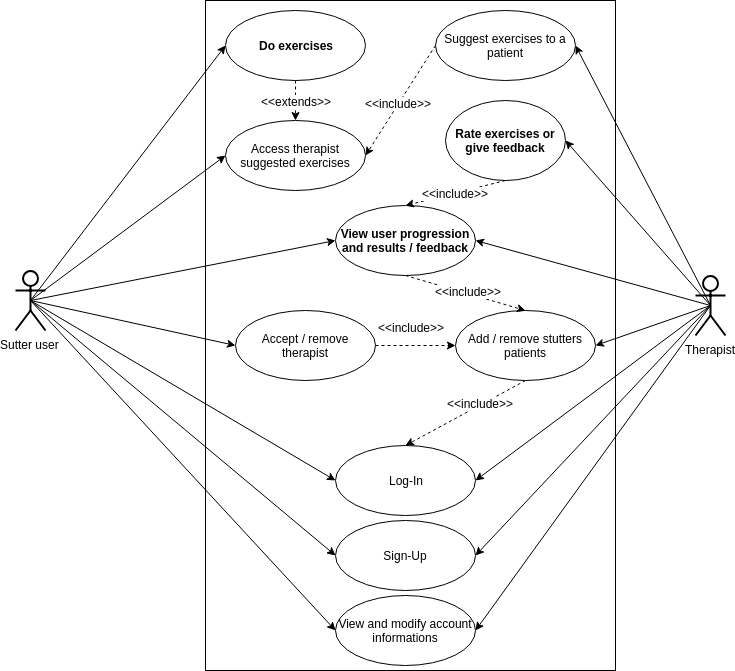
\includegraphics[width=.9\linewidth]{content/imgs/usecase.png}
  \caption{Diagramme cas d'utilisation}
  \label{fig:srs}
\end{figure}

\subsection{Résumé de cahier des charges de l'application}
\label{sec:resume_cdc}

L'application est destiné à être utilisé par des personnes souffrant de bégaiement et par des orthophonistes. Au premier démarrage de l'application l'utilisateur devra alors choisir s'il souhaite utilisé l'application en tant que bègue ou en tant qu'orthophoniste.

\subsubsection{Utilisateurs bègues}

Les bègues auront à disposition une liste d'exercices pour s'entrainer à mieux contrôler leurs flux de parole. Chaque exercice sera paramétrable pour convenir aux besoins de l'utilisateur. En particulier, les exercices pourront utiliser des ressources que l'utilisateur devra lire. Ces ressources devront être récupérées via une collection de ressources partagée possédant plusieurs type de ressources : des mots, des phrases et des textes. Le bègue pourra alors choisir sur quelle type de ressource il veut s'entrainer. Les exercices pourront s'appuyer aussi sur d'autres éléments, par exemple un enregistreur vocale ou vidéo pour enregistrer l'exercice. L'utilisateur pourra choisir d'activé ou non ces enregistreurs. Voici 4 exercices types qui rentre dans le cadre de l'application :

\begin{itemize}
  \item \textbf{Metronome} : le bègue s'entraine à parler avec un rythme régulié grâce à un metronome (appareil émettant un signal -- visuel et/ou sonor -- à interval de temps régulier) ;
  \item \textbf{Reading} : le bègue parle librement sur des ressources de son choix (mot, texte, phrase) ;
  \item \textbf{Delayed Auditory Feedback (DAF)} : le bègue parle puis entend le retour de sa voix quelques dizaines de millisecondes après ;
  \item \textbf{Mirroring} : le bègue s'entraine à parler avec un retour vidéo de sa tête pour analyser ses mouvements faciales.
\end{itemize}

L'utilisateur bègue pourra accéder à sa progression. La progression est consituée de l'historique de tous les exercices effectués. Ces exercices contiendront l'eventuel enregistrement vocale ou vidéo, les ressources utilisées lors de l'exerice ainsi qu'un commentaire de son éventuel orthophoniste (voir ci-après). La progression de l'utilisateur devra aussi pouvoir être visualisée graphiquement grâce à une courbe illustrant le pourcentage de réussite de prononciation des mots prononcés lors des exercices.

L'utilisateur bègue pourra décider de synchroniser ses exercices dans le cloud. Pour ce faire il devra se créer un compte avec un nom, une adresse mail et un mot de passe. Une fois un exercice synchronisé dans le cloud, il sera accessible par son éventuel orthophoniste qui pourra alors ajouter un commentaire sur cet exercice. Les utilisateurs bègues peuvent donc ajouter un orthophonistes autorisé à avoir accès à tous leurs exercices synchronisés. Pour ajouter un orthophoniste ils devront connnaitre son identifiant personnel (voir ci-après). Ils pourront bien entendu révoquer l'accès de cet orthophoniste aux exercices à tout moment.

\subsubsection{Utilisateurs orthophonistes}

Pour utiliser les fonctionnalités de l'application, les orthophonistes devront créer un compte (comme pour les bègues, avec un nom d'utilisateur, un courriel et un mot de passe). Une fois le compte créé, l'orthophoniste aura accès à son identifiant personnel ainsi que le liste de tous les utilisateurs bègues l'ayant ajouté comme orthophoniste. Ces utilisateurs son appelé \textit{patients} pour l'orthophoniste. L'orthophoniste pourra visualiser la progression des ses patients. Il pourra aussi supprimer des patients de sa liste.















% eof
